\section{Experimental Results}
\label{exp}

\begin{figure}
    \centering
    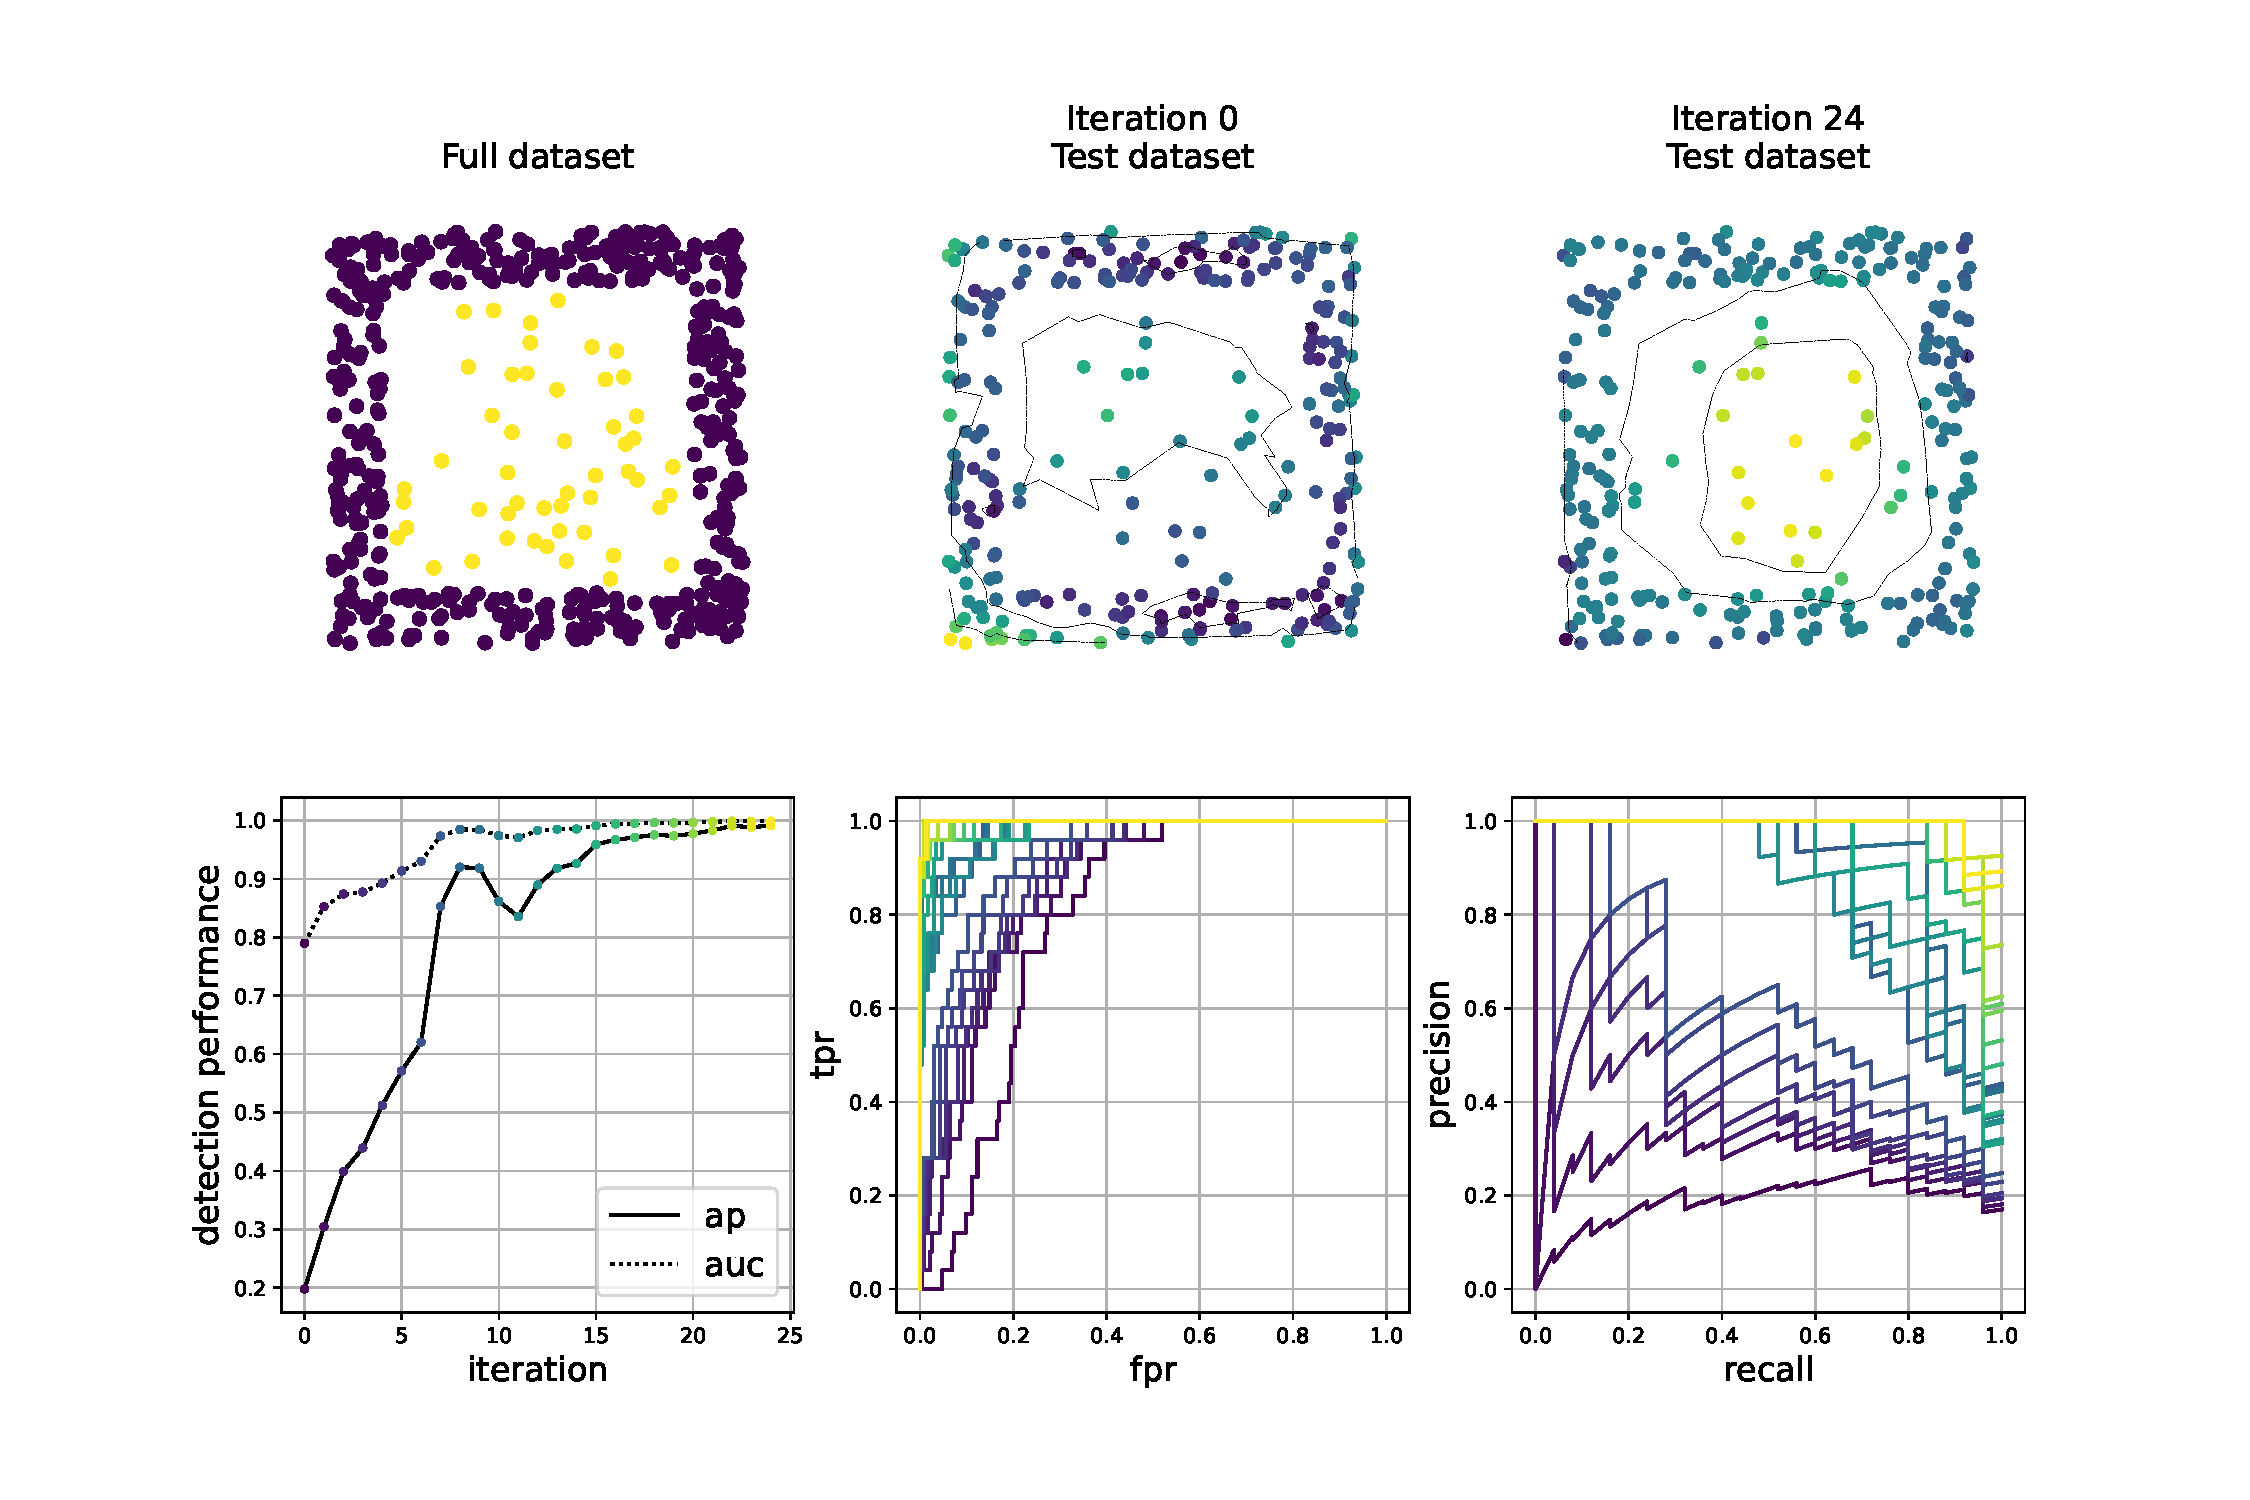
\includegraphics[width=\textwidth]{square_toroid_6fig.pdf}
    \caption{Test of the algorithm on a square toroidal dataset: anomalies lie inside of a box made up of normal instances. This setting is particularly challenging for the Isolation Forest algorithm as it is much easier to quickly separate normal points (depicted in purple) w.r.t anomalies (yellow). The anomaly score on test samples is shown on the second and third panel: the yellow is assigned to the points having the highest anomaly score, the purple viceversa. In the second row of panels the performances of the detector at each iteration is depicted: the \emph{area under the ROC curve} (auc) and the \emph{average precision} (ap) measured on the test set quickly improve. }
    \label{fig:toroid}
\end{figure}

%\begin{figure}
%    \centering
%    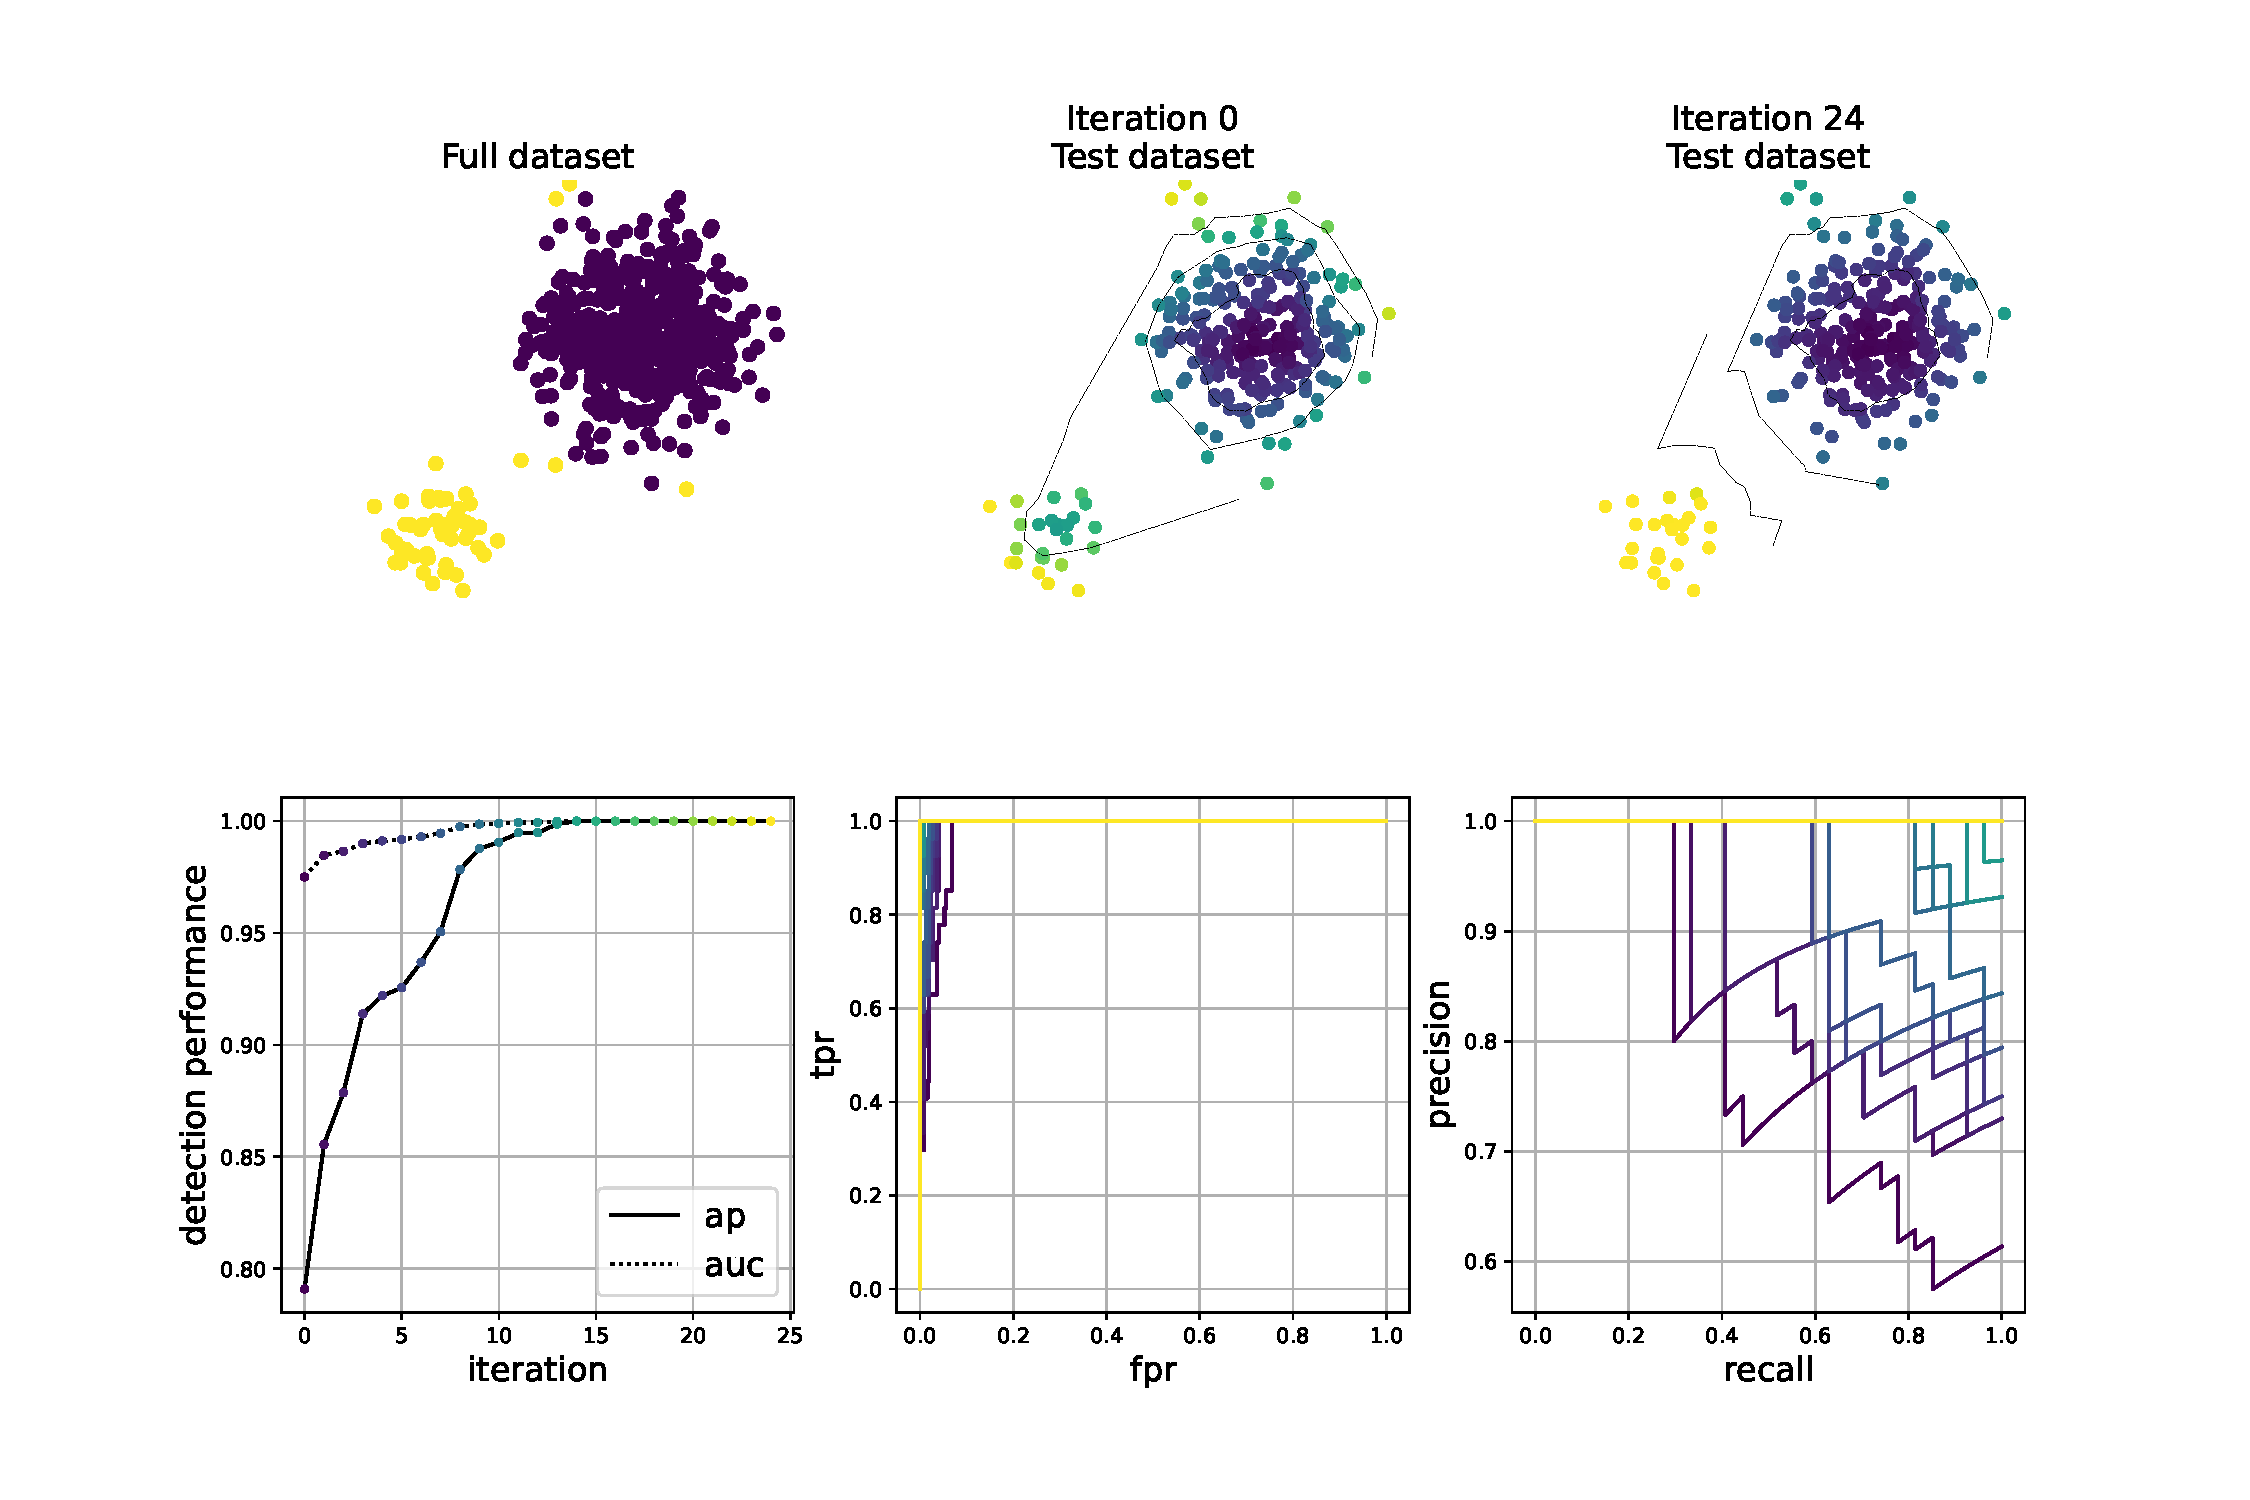
\includegraphics[width=\textwidth]{images/anomalous_cluster_6fig.pdf}
%    \caption{ciao ciao ciao}
 %   \label{cluster}
%\end{figure}

%tabella dei dataset
%descrizione dataset
In this section,  we analyse the performance of \approach, matching both the proposed update strategies with the two described query approaches. Doing so, we hope to obtain a full and detailed evaluation of the presented model, with the purpose of analysing the efficiency of each combination as well as giving meaningful guidance on the proper use of the proposed strategies.
%This section describes the achieved results obtained using the two query strategies proposed in the previous section. Specifically, we match the proposed fixing strategy together with the two query strategies, in order to obtain a full and detailed evaluation of the presented model. 

%The proposed model performance is compared with the Isolation Forest as well as with the Random Forest. Our approach, in fact, essentially relies on designing an active learning based modification of the classical Isolation Forest. Therefore, since, even if of a small size, we are now dealing with a labeled set of data, we decided it was fair to compare the proposed approach with a supervised learning model. Specifically, we picked the Random Forest on account of its binary tree based structure.

Firstly, we tested our approach on synthetic datasets like the challenging shape depicted in Figure \ref{fig:toroid}, where the normal data make up a square toroid and the anomalous data lie inside it. In this kind of datasets, the Isolation Forest perform quite badly and there is a lot of room for improvement as it struggles to  separate in few steps the anomalies: in this case it is much easier to wrongly separate normal points w.r.t. anomalies, indeed the first iteration of the model corresponding to the unsupervised training gives the highest anomaly score to the normal bottom left point of the toroid. On the contrary, at the 25-\textit{th} iteration the model has learnt the correct function and is able to perfectly classify all the points. This is also visible in the panels of the second row of Figure \ref{fig:toroid}, where the performance of the detector at each iteration is depicted with lines having different colors. As the model is allowed to query new points, the average detection performance quickly improves.

We decided to test the model on a set of $18$ real data openly available \cite{Rayana,Dua:2019}.
Table \ref{dataset_used} presents the dataset used to test the performance of the proposed model. These come from different domains like medicine, industry and natural sciences and are characterised by various number of points as well as percentage of anomalous data. Defining the contamination as the ratio between the number of anomalies and total number of samples of the dataset, they are characterized by a wide feature range between $6$ to $100$ and a contamination percentage between $0.9\%$ and $36\%$. It is very important to highlight how most of these datasets were built: they are adaptations of multi-class classification datasets to the anomaly detection task where one of the classes is under sampled and labelled as outlier. This means that points considered outliers are not just points randomly scattered in the features space like general anomalies, but they live in specific positions of the space that can be hard to be defined without labels. In this context, weakly supervised methods prove their efficacy, starting from an unsupervised guess, and improving continuously as labels are included in the model.

\begin{table*}[]
\centering
	\begin{tabular}{@{}lccc c@{}} \hline
		\textbf{Dataset} & \textbf{Instances} & \textbf{Features} & \textbf{Anomalies}  & \textbf{Contamination}\\ \hline
		AnnThyroid   & 7200                & 6                  & 534        & 7.42\%        \\ 
		Breastw      & 683                 & 9                  & 239        & 35 \%        \\
		Cardio &	1831 & 21 & 176 & 9.6\% \\
		Cover & 286048 & 10 & 2747 & 0.9\% \\
		Ionosphere   & 351                 & 33                 & 126          &      36\%\\
		Letter & 1600 &  32 & 100 & 6.25\% \\
		Mammography  & 11183               & 6                  & 260           &  2.32\%   \\
		Mnist & 7603 & 100 & 700 & 9.2\% \\
		Optdigits	& 5216 & 64 &	150 & 3\% \\
		Pendigits    & 6870                & 16                 & 156          &  2.27\%    \\
		Pima         & 768                 & 8                  & 268          &  35\%    \\
		Satellite & 6435 & 36 & 2036  & 32\% \\
		Satimage-2	&5803&36&	71& 1.2\% \\
		Thyroid	& 3772 & 6 & 93 & 2.5\% \\
		Vertebral	&240&	6	&30 &12.5\% \\
		Vowels& 	1456&12	&50 &3.4\%   \\
		WBC	&278	&30	&21 &5.6\%   \\ 
		Wine & 129	& 13	& 10 & 7.7\% \\ \hline
		
	\end{tabular}
	\caption{Set of data used in the experimental phase. The first column gives the name of the dataset; the second column describes the number of instances contained in each set; the third column defines the total amount of features; the fourth column gives the number of outliers; the last column presents the contamination rates.}
	\label{dataset_used}
	\end{table*}

We used the average precision score metric to measure the results obtained. Splitting equally the dataset in training and testing set, we carried on a number of $25$ queries, and the experiments were conducted $50$ independent times to study the performances distribution. 
The experiments were performed on equipment with Intel Core i7-6800K CPU and 32 GB RAM. The implementation of \approach is freely available online\footnote{\url{https://github.com/tombarba/ActiveLearningIsolationForest} }. 

First, we tested the four possible combinations of the two proposed update strategies together with the two query strategies so as to determine the best combination with respect to the majority of the considered test sets. Figure \ref{risultati_1} shows the obtained results.

%why credibility has problems
\begin{figure*}
   \centering
    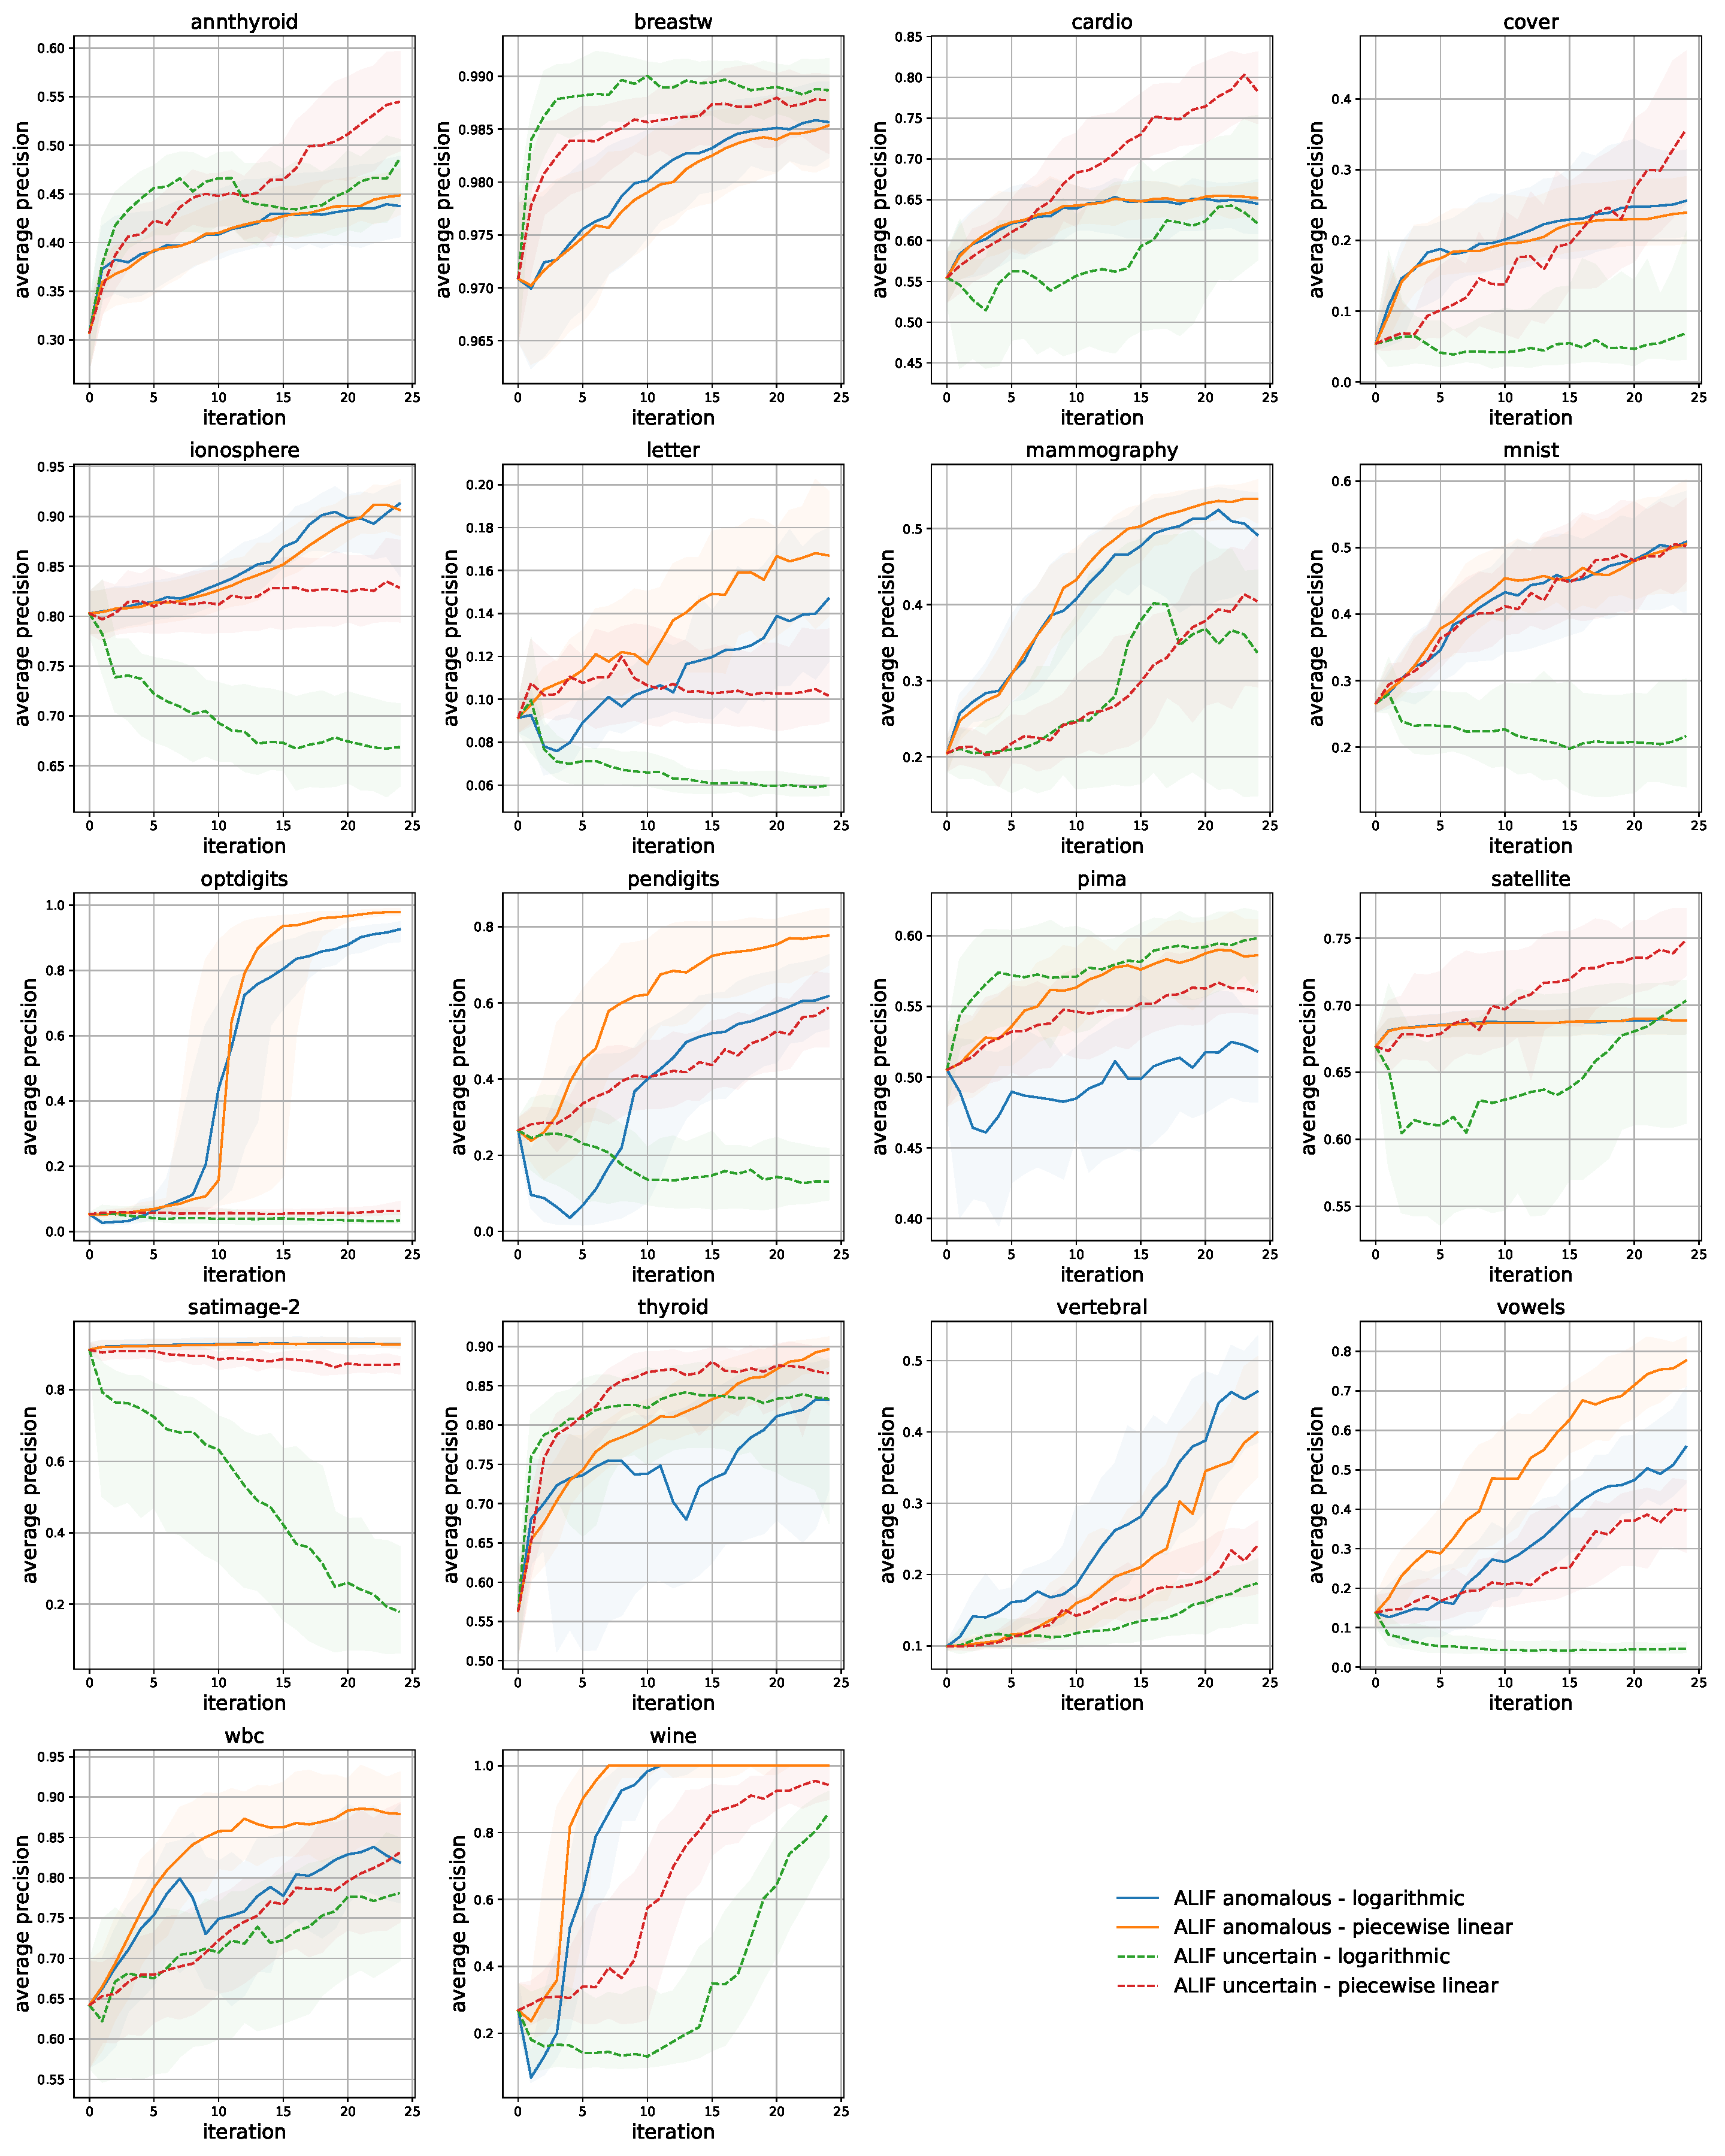
\includegraphics[width=\textwidth]{four_strategies.pdf}
    \caption{Performance of the four combinations of the proposed strategies with the datasets described in Table \ref{dataset_used}. As a general result, it can be noticed that querying the most anomalous point represents the most appropriate choice, overall leading to quicker improvements of the performance. When it comes to the update strategies, both the linear and the logarithmic depths seem to represent a reasonable choice. However, the linear depth appears to moderately be more stable.}
    \label{risultati_1}
\end{figure*}

%\tommi{un commento dei revisori potrebbe essere: mi mostri anche la query randomica?} \gas{concordo}
% 4 approcci
Given that the first point of the curve represents the performance of the fully unsupervised Isolation Forest, it can be observed as, broadly speaking, all four proposed matches represent an improvement with respect to the performance of the Isolation Forest. The two trials of the "most anomalous" query are depicted in solid line, while the "maximum uncertainty" in dashed line. Even if there are some exceptions, in most cases the first policy seems the one having the fastest improvements. This is a very interesting aspect since the "most anomalous" strategy is the cheapest and most natural policy among the two considering the DSS scenario previously described. Concerning the updating strategy, as expected, the piece-wise linear is the one having the most stable improvements in the dataset and among the datasets. As a direct consequence, we decided to use the combination "most anomalous - piecewise linear" for the comparison to the other baseline and state-of-art competitor.

% state-of-art
As our approach \approach essentially relies on designing an active learning based modification of the classical Isolation Forest, we decided to compare it with other tree based models: a fully supervised model, i.e. the Random Forest, and a weakly supervised model, the Isolation Forest - Active Anomaly Detection (IF-AAD).
The RF represents the baseline since it is the most well known but simple classification approach; unfortunately it requires samples from both the classes inlier/outlier and it is computationally expensive as every time the user labels a new data point the forest is retrained. As the RF does not have a default method to query its points, in the following comparison the points given to the RF for training are the points queried by our \approach.
On the other side IF-AAD is a active semi-supervised model  that does not need both class labels and is available online\footnote{\url{https://github.com/shubhomoydas/ad_examples}}. 

\begin{figure}
    \centering
    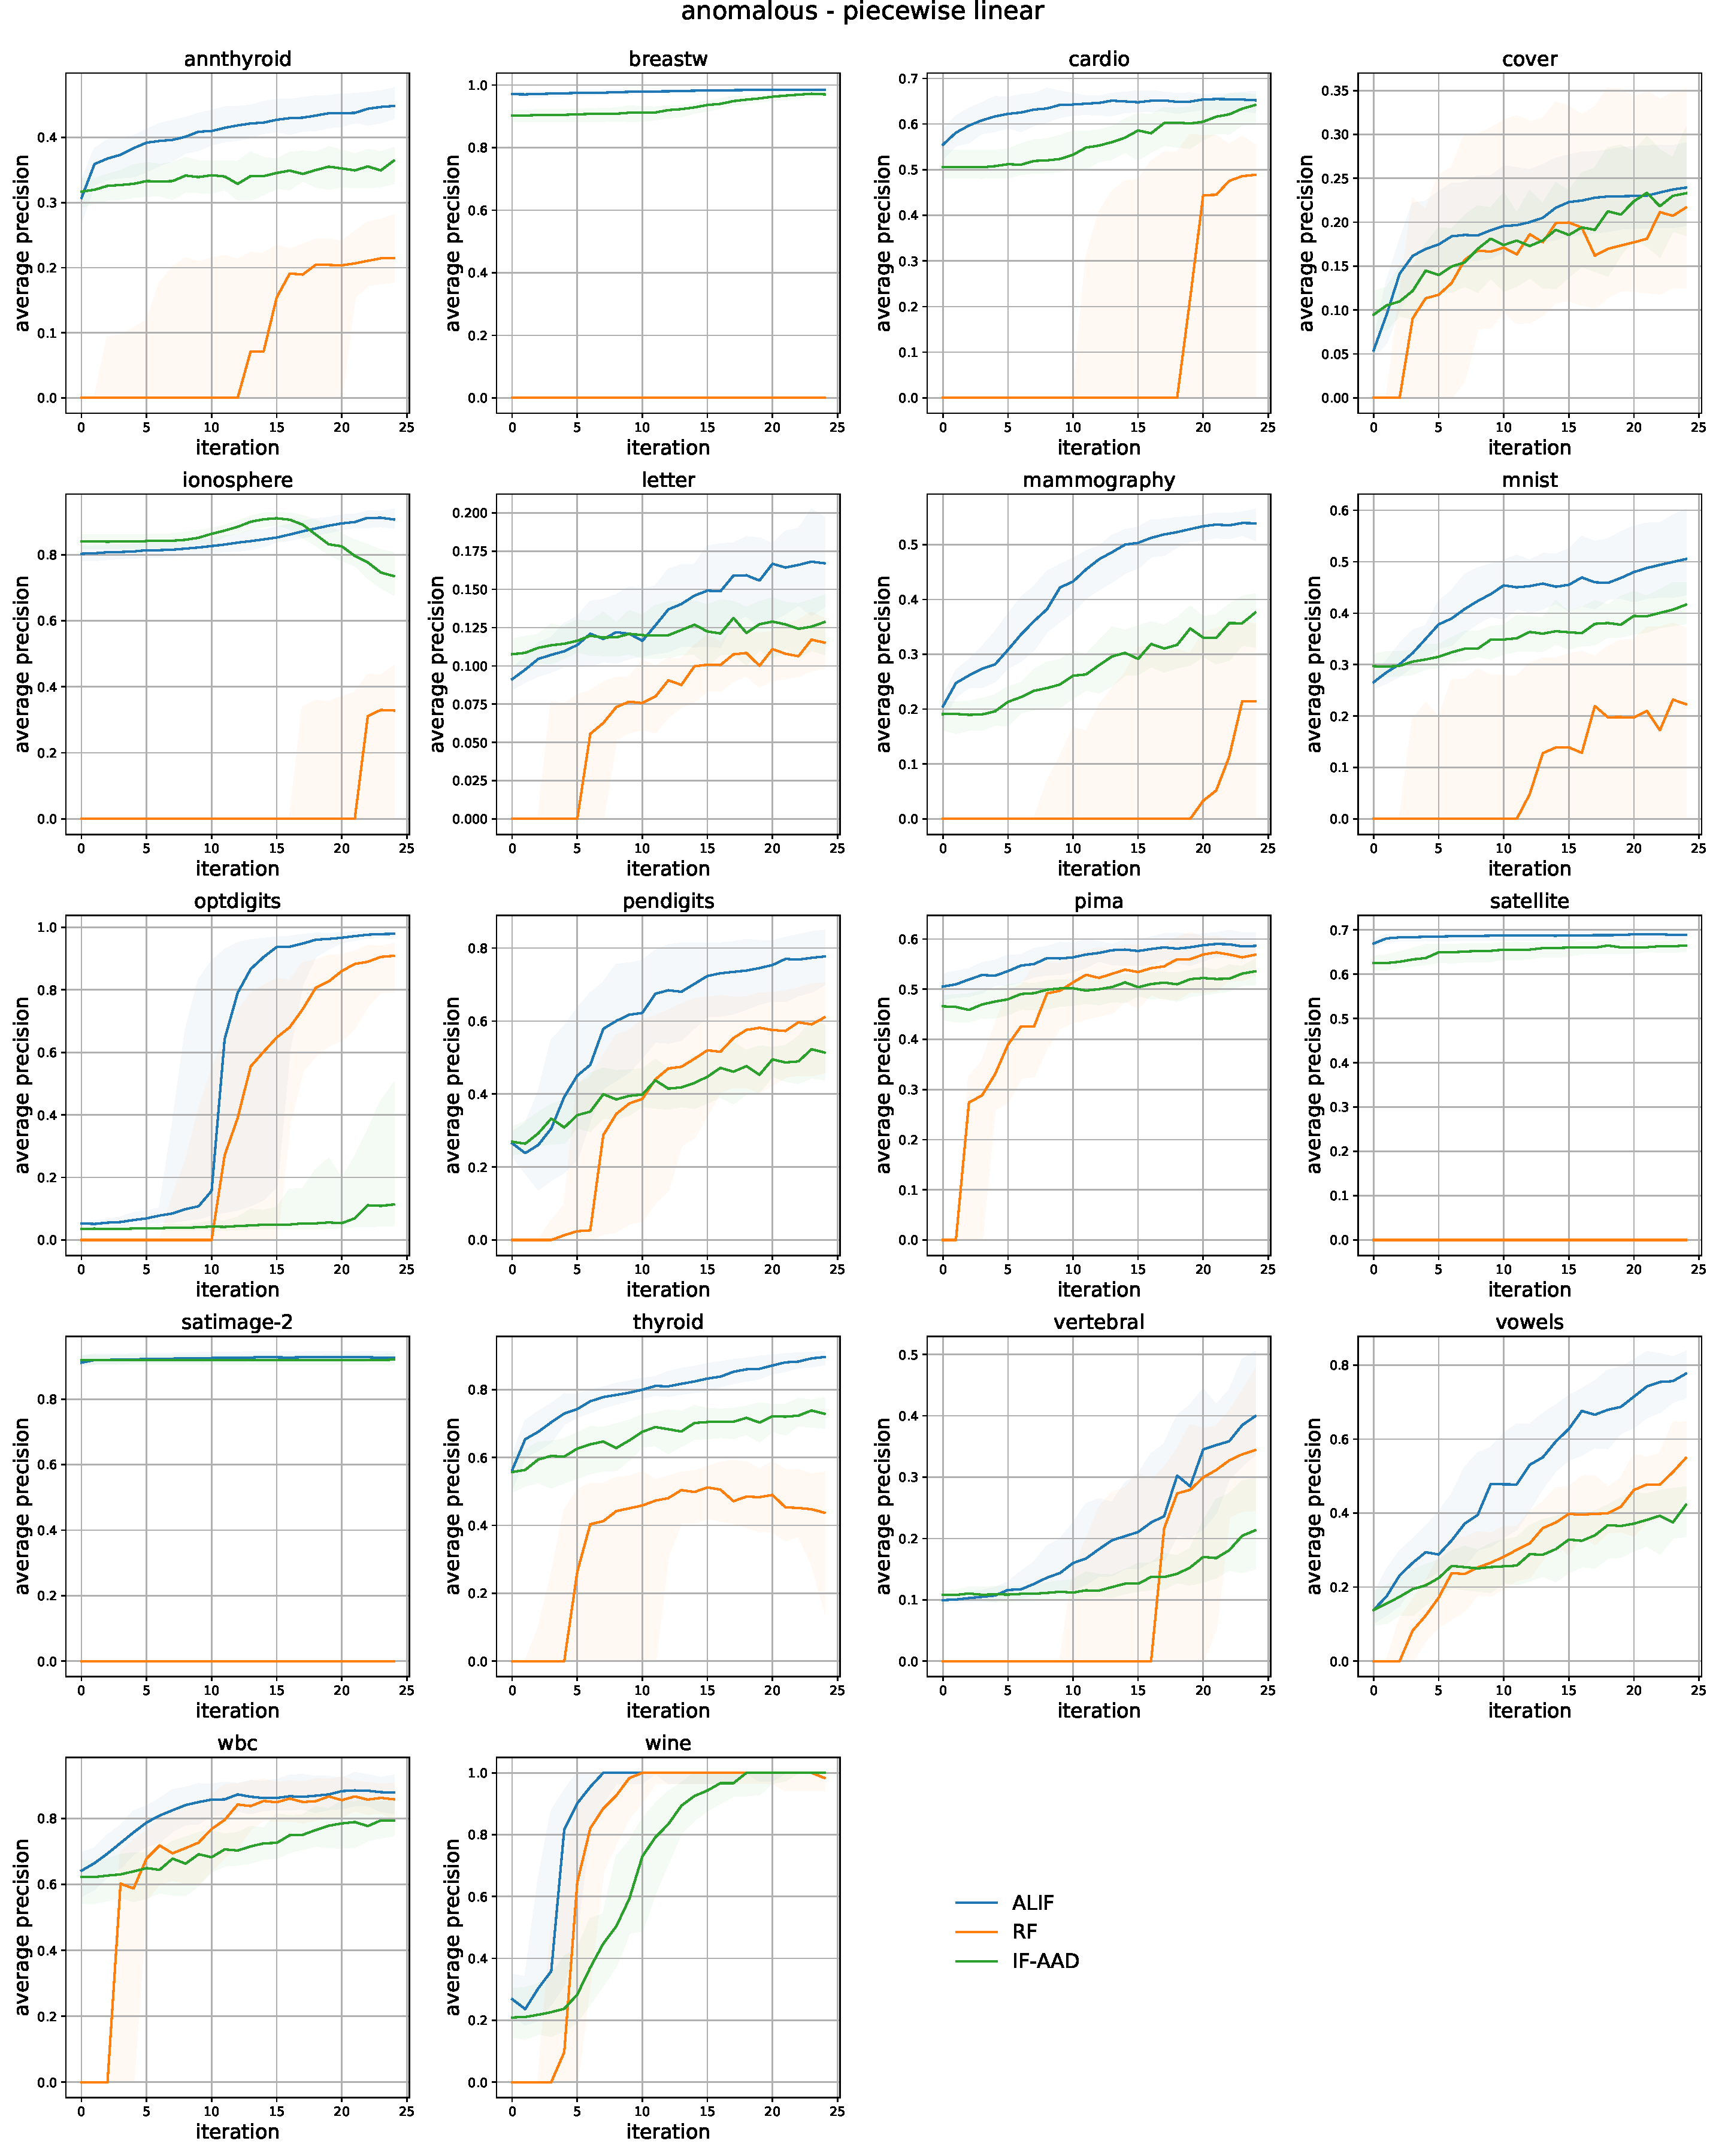
\includegraphics[width=\textwidth]{anomalous_piecewise.pdf}
    \caption{Comparison of most anomalous - piece-wise linear \approach with IF-AAD and RF. It can be observed that, in general our method represents the best course of action, having the highest performance score usually with a very small amount of labeled data.}
    \label{benchmark}
\end{figure}

Figure \ref{benchmark} and Table \ref{table:final_results} show the benchmark results: it is prominent that \approach obtains the finest results with a very little number of labels, generally outperforming IF-AAD. Due to the strong imbalance between inliers and outliers RF receives quite late both labels from the two classes, leading to poor detection performances: in \emph{breastw}, \emph{satellite}, and \emph{satimage-2} the querying process never got them over 25 iterations and 50 independent repetitions %\tommi{questi sarebbero stati tutti falsi positivi comunque}.



\begin{table}[]
\centering
\begin{adjustbox}{angle=270}
\begin{tabular}{llllllllll}
\toprule
{} &      {}  & \multicolumn{2}{l}{anom-log} & \multicolumn{2}{l}{anom-lin} & \multicolumn{2}{l}{unc-log} & \multicolumn{2}{l}{unc-lin} \\
{} & IF-AAD &       RF &   ALIF &       RF &   ALIF &      RF &   ALIF &      RF &   ALIF \\
\midrule
\textbf{annthyroid } &   0.34 &     0.11 &  0.41 &     0.11 &  0.41 &    0.11 &  0.44 &    0.22 &  \textbf{0.45} \\
\textbf{breastw    } &   0.93 &     0.00 &  0.98 &     0.00 &  0.98 &    0.28 &  \textbf{0.99} &    0.48 &  0.98 \\
\textbf{cardio     } &   0.56 &     0.15 &  0.63 &     0.16 &  0.63 &    0.34 &  0.57 &    0.49 &  \textbf{0.69} \\
\textbf{cover      } &   0.18 &     0.20 &  0.21 &     0.18 &  0.20 &    0.25 &  0.09 &    \textbf{0.46} &  0.19 \\
\textbf{ionosphere } &   0.84 &     0.08 &  \textbf{0.85} &     0.08 &  \textbf{0.85} &    0.47 &  0.70 &    0.52 &  0.82 \\
\textbf{letter     } &   0.12 &     0.08 &  0.11 &     0.07 &  \textbf{0.14} &    0.06 &  0.07 &    0.07 &  0.11 \\
\textbf{mammography} &   0.28 &     0.09 &  0.40 &     0.10 &  \textbf{0.43} &    0.04 &  0.28 &    0.18 &  0.28 \\
\textbf{mnist      } &   0.36 &     0.15 &  0.41 &     0.15 &  \textbf{0.43} &    0.25 &  0.24 &    0.42 &  0.42 \\
\textbf{optdigits  } &   0.11 &     0.46 &  0.49 &     0.38 &  \textbf{0.51} &    0.00 &  0.05 &    0.00 &  0.06 \\
\textbf{pendigits  } &   0.42 &     0.28 &  0.39 &     0.34 &  \textbf{0.59} &    0.10 &  0.19 &    0.24 &  0.42 \\
\textbf{pima       } &   0.50 &     0.44 &  0.49 &     0.43 &  0.56 &    0.34 &  \textbf{0.57} &    0.43 &  0.54 \\
\textbf{satellite  } &   0.65 &     0.01 &  0.69 &     0.01 &  0.68 &    0.42 &  0.64 &    0.49 &  \textbf{0.70} \\
\textbf{satimage-2 } &   0.92 &     0.00 &  \textbf{0.93} &     0.00 &  \textbf{0.93} &    0.25 &  0.48 &    0.53 &  0.88 \\
\textbf{thyroid    } &   0.66 &     0.37 &  0.69 &     0.33 &  \textbf{0.80} &    0.10 &  0.73 &    0.33 &  \textbf{0.80} \\
\textbf{vertebral  } &   0.14 &     0.16 &  \textbf{0.27} &     0.12 &  0.22 &    0.17 &  0.14 &    0.22 &  0.17 \\
\textbf{vowels     } &   0.29 &     0.29 &  0.33 &     0.30 &  \textbf{0.51} &    0.07 &  0.06 &    0.18 &  0.27 \\
\textbf{wbc        } &   0.71 &     0.68 &  0.76 &     0.68 &  \textbf{0.82} &    0.11 &  0.69 &    0.21 &  0.73 \\
\textbf{wine       } &   0.69 &     0.73 &  0.80 &     0.75 &  \textbf{0.85} &    0.28 &  0.38 &    0.47 &  0.64 \\
\bottomrule
\end{tabular}
\end{adjustbox}

\caption{Summary of the obtained results. The reported performances are the mean performance along the 25 iterations and 50 repetitions of the algorithm. \approach consistently beats the other tested approached on all the datasets, in particular the combination of the most anomalous query policy and the piece-wise linear leaf update.}
\label{table:final_results}
\end{table}

%\gas{C'e' altro di sperimentale che possiamo mostrare? La Fig. 4 e 5 sono ottime, ma se vi viene in mente altro (il paper non e' lunghissimo al momento) non guasterebbe}




%\tommi{domani ci lavoro su}
%\begin{figure}
%    \centering
%    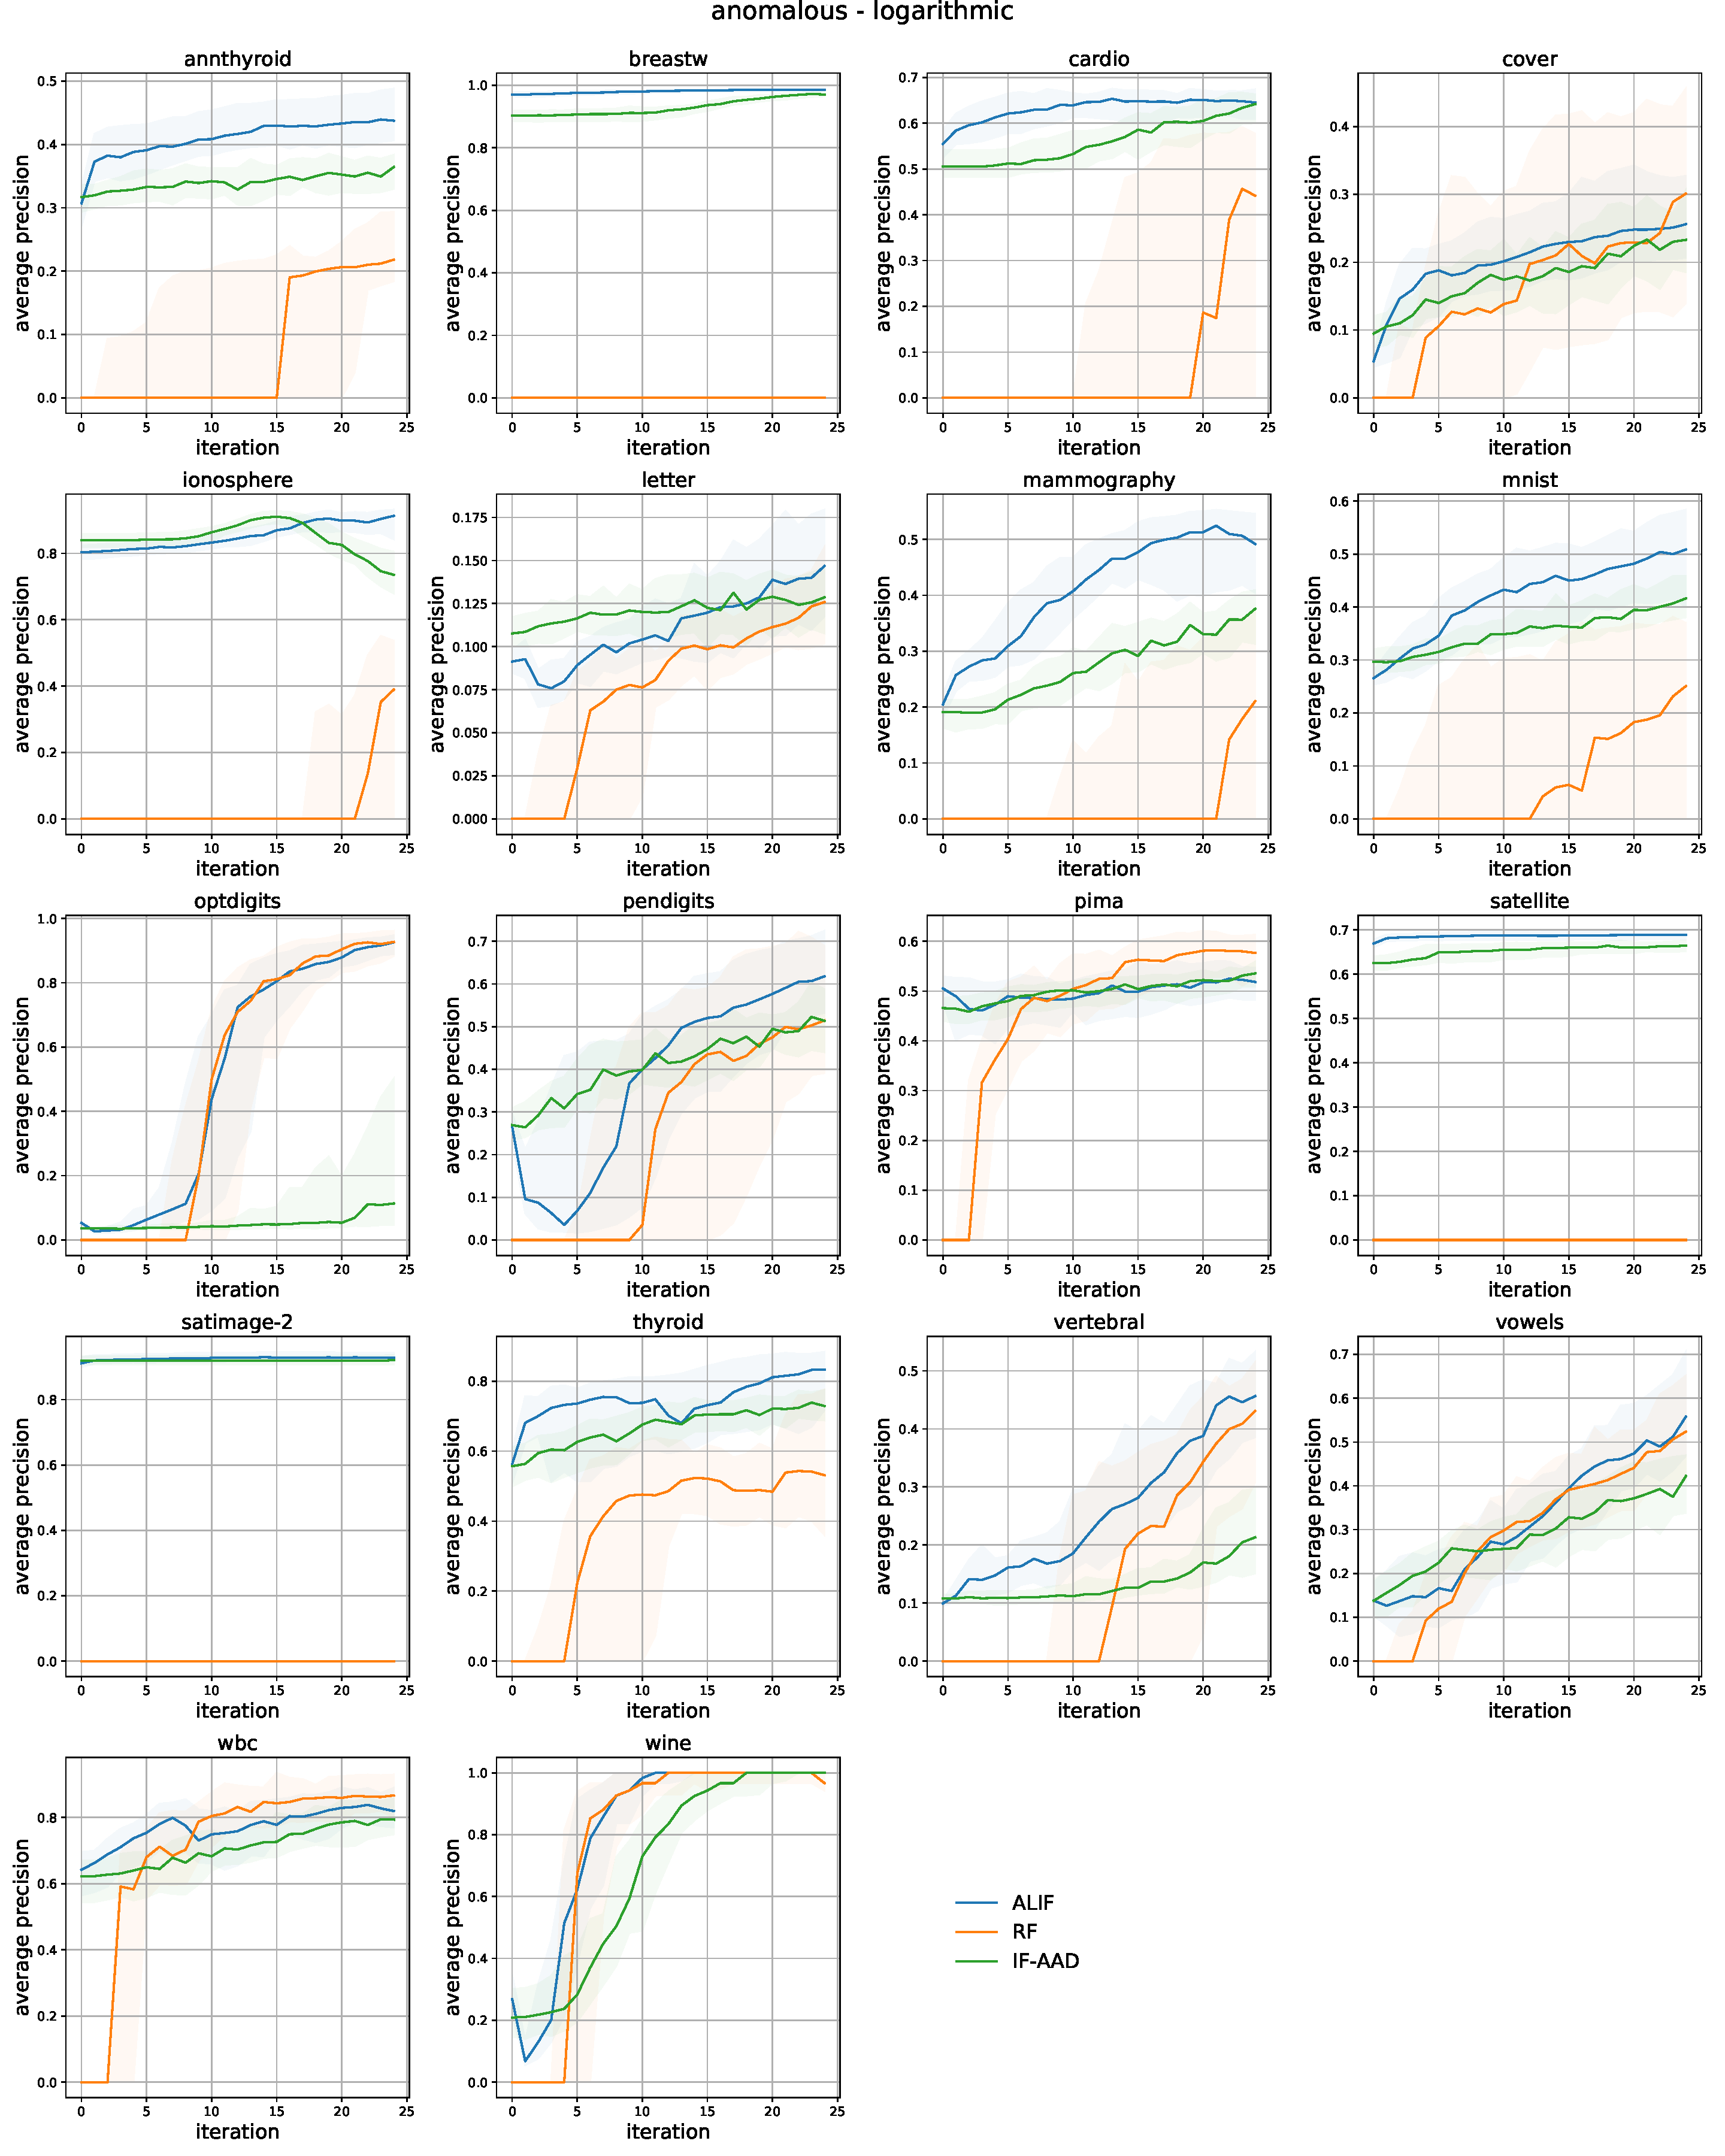
\includegraphics[width=\textwidth]{images/anomalous_log.pdf}
%    \caption{Comparison of most anomalous - logarithmic ALBIF with IF-AAD and RF. As for the most anomalous - piece-wise combination shown in Figure \ref{benchmark}, ALBIF often has the highest performance score having a very small amount of labeled data at disposal.}
%    \label{benchmark2}
%\end{figure}